\documentclass[9pt]{beamer}
\usepackage{silence}
\WarningFilter{beamerthememetropolis}{You need to compile with XeLaTeX or LuaLaTeX to use the Fira fonts}
\usetheme[titleformat = smallcaps, block = fill, progressbar = frametitle]{metropolis}
\title{\huge \mbox{Elements of Mathematics - Exercises}}
%---------------------------------%
% PACKAGES
%---------------------------------%
% Input encoding.
\usepackage[utf8]{inputenc} % For accents in spanish: transforms "á" into "\'a"
\usepackage[T1]{fontenc} % Output encoding. Use to avoid silly problems on the output.
                         % See: http://tex.stackexchange.com/questions/664/why-should-i-use-usepackaget1fontenc
\usepackage[sfdefault]{FiraSans}
\usepackage{FiraMono}
% AMS packages
\usepackage{amsmath}
\usepackage{amsfonts}
\usepackage{amssymb}
\usepackage{amsthm}
% Matrices
\usepackage{mathtools}
\newcommand{\verteq}{\rotatebox{90}{$\,=$}}
\usepackage{gauss}
% Customization for augmented matrices; 
% see https://tex.stackexchange.com/questions/146723/how-to-typeset-row-operations-on-augmented-matrix
% Patch gauss macros for doing their work in `align'
% and other amsmath environments; see http://tex.stackexchange.com/questions/146532/
\usepackage{etoolbox}
\makeatletter
\patchcmd\g@matrix
    {\vbox\bgroup}
    {\vbox\bgroup\normalbaselines} % restore the standard baselineskip
    {}{}
\makeatother
\newcommand{\BAR}{%
    \hspace{-\arraycolsep}%
    \strut\vrule % the `\vrule` is as high and deep as a strut
    \hspace{-\arraycolsep}%
}
% Math blackboard font
\usepackage{bbm}
% Fonts
\usepackage{lmodern} 
% \usepackage[sfdefault]{FiraSans}
\usepackage[normalem]{ulem}
\usepackage{eulervm}
% Graphics
\usepackage{graphicx} 
\usepackage{float}
\usepackage{subcaption}
\usepackage{wrapfig}
\usepackage{animate}
\usepackage{caption}
% Algorithms
\usepackage[ruled]{algorithm2e}
\newcommand{\lIfElse}[3]{\lIf{#1}{#2 \textbf{else}~#3}}
% Boxes
\usepackage[most]{tcolorbox}
% For reference enumerations lists
\usepackage{enumitem}
% \setlist{labelwidth = \widthof{0.}, leftmargin = {\labelwidth+\labelsep}, 
%         rightmargin = \leftmargin} % Setting left marging = right marging in itemize envirnment
% Import icons
\usepackage{fontawesome}
% Hyperlink
\usepackage{hyperref}
\hypersetup{
	final,
    bookmarksnumbered=true,
    bookmarksopen=true,
    bookmarksopenlevel=0,
    unicode=false,          % non-Latin characters in Acrobat?s bookmarks
    pdftoolbar=true,        % show Acrobat?s toolbar?
    pdfmenubar=true,        % show Acrobat?s menu?
    pdffitwindow=false,     % window fit to page when opened
    pdftitle={Introduction to Mathematics},    % title
    pdfdisplaydoctitle=true, %display document title instead of file name in title bar
    pdftoolbar=true,
    pdfmenubar=true,
    pdflang={English},
    pdfauthor={Abel Guada Azze},     % author
    pdfsubject={Introduction to Mathematics},   % subject of the document
    pdfcreator={Abel Guada Azze},   % creator of the document
    pdfproducer={Abel Guada Azze}, % producer of the document
    pdfkeywords={Mathematics} {introduction}, % list of keywords
    pdfnewwindow=true,      % links in new window
    breaklinks=true,
    hidelinks,
    colorlinks,
    linkcolor=black,          % color of internal links (change box color with linkbordercolor)
    citecolor=black,        % color of links to bibliography
    filecolor=cyan,      % color of file links
    urlcolor=magenta           % color of external links
}
%----------------------------------- Tikz
\usepackage{tikz}
\usepackage{pgfplots}
% \pgfplotsset{compat=1.18}
% \usepackage{tkz-euclide}
\usetikzlibrary{shapes,arrows.meta,matrix,positioning,calc}
\newcommand{\tikzmark}[1]{\tikz[baseline,remember picture] \coordinate (#1) {};}
% ---------- Helpers: 2-set and 3-set Venns ----------
% \VennTwoCounts{LabelA}{LabelB}{onlyA}{both}{onlyB}{Neither}{Universe}
\newcommand{\VennTwoCounts}[7]{%
  \begin{tikzpicture}[scale=1.0,baseline=(current bounding box.center)]
    \def\r{1.8}   % circle radius (cm)
    \def\dx{2.35} % distance between centres (cm)
    \def\pad{0.60} % padding between circles and rectangle (cm)

    \coordinate (A) at (0,0);
    \coordinate (B) at (\dx,0);

    % Universe rectangle (outline only)
    \draw[line width=.8pt, rounded corners=2pt]
      ($(A)+(-\r-\pad,-\r-\pad)$) rectangle ($(B)+(\r+\pad,\r+\pad)$);

    % Set fills + outlines
    \fill[black!8] (A) circle (\r);
    \fill[black!8] (B) circle (\r);
    \draw[line width=.8pt] (A) circle (\r);
    \draw[line width=.8pt] (B) circle (\r);

    % Universe label (top-left inside the box)
    \node[font=\scriptsize,anchor=north west]
      at ($(A)+(-\r-\pad+0.12,\r+\pad-0.12)$) {#7};

    % Set labels
    \node[font=\small\bfseries] at ($(A)+(0,0.68*\r)$) {#1};
    \node[font=\small\bfseries] at ($(B)+(0,0.68*\r)$) {#2};

    % Counts
    \node[font=\small] at ($ (A)+(-0.60*\r,-0.05*\r) $) {#3}; % only A
    \node[font=\small] at ($ .5*(A)+.5*(B) $) {#4};           % both
    \node[font=\small] at ($ (B)+(0.60*\r,-0.05*\r) $) {#5};  % only B
    \node[font=\small]
      at ($ (B)+(\r+0.3*\pad,0.78*\r) $) {#6};                % outside
  \end{tikzpicture}%
}


%---------------------------------%
% Biblio
%---------------------------------%

%---------------------------------%
% SETTINGS
%---------------------------------%
% displays sections and subsections numbered in the TOC
\setbeamertemplate{section in toc}[sections numbered]
% \setbeamertemplate{subsection in toc}[subsections numbered]
% gets rid of bottom navigation bars
\setbeamertemplate{footline}{}
% gets rid of bottom navigation symbols
\setbeamertemplate{navigation symbols}{}
% sets images' path
\graphicspath{{img/}}
% resets footnote counter at the beginning of each section
\AtBeginEnvironment{frame}{\setcounter{footnote}{0}}
% beamer margins
\setbeamersize
{
    text margin left=3mm,
    text margin right=3mm,
    % sidebar width left=.0cm,
    % sidebar width right=.0cm,
    % description width,
    % description width of=,
    % mini frame size=,
    % mini frame offset
}
% redefines block environment to add small space between title and content
\let\oldblock\block
\let\endoldblock\endblock
\renewenvironment{block}[1]
    {\begin{oldblock}{#1}
        \vspace{0.1cm}
    }
    { 
    \end{oldblock}
    }

%---------------------------------%
% SETTINGS
%---------------------------------%
%---------------------------------%
% TITLE PAGE
%---------------------------------%
\setbeamertemplate{title page}{
    \vspace{-0.4cm}
    
    \textcolor{CUNEForange}{\rule{\textwidth}{0.05cm}}
    \vspace{-0.65cm}
    
    \begin{minipage}{0.2\textwidth}
        \includegraphics[width = 2.0cm]{Logo-CUNEF.png}
    \end{minipage}
    \begin{minipage}{0.7\textwidth}
        
        \quad \Huge \usebeamertemplate*{title}
        
    \end{minipage}    
    \vspace{-0.25cm}
    
    \textcolor{CUNEForange}{\rule{\textwidth}{0.05cm}}
    \vspace{1.5cm}

    \begin{minipage}{0.075\textwidth}
        
    \end{minipage}\hfill\textcolor{CUNEForange}{\vrule\vrule\vrule}
    \begin{minipage}{0.825\textwidth}
        \begin{itemize}[leftmargin = *, label= $ $]
            \item {\hspace{1.05pt} \faUser\quad Abel Guada Azze}
            \item {\hspace{0pt} \faEnvelope\quad \href{mailto:abel.guada@cunef.edu}{abel.guada@cunef.edu}}
            \item {\hspace{0pt} \faSuitcase\quad F4.5 - C. de Leonardo Prieto Castro, 2}
            \item {\hspace{0pt} \faUniversity\ \ \ Department of Quantitative Methods - CUNEF Universidad}
            \item {\hspace{0pt} \faGraduationCap\ \ \ Bachelor in Philosophy, Politics and Economics}
        \end{itemize}
    \end{minipage}
}
\setbeamertemplate{title}{
  \linespread{1.0}%
  \inserttitle%
  \par%
  \vspace*{0.5em}
}
\setbeamertemplate{subtitle}{
  \insertsubtitle%
  \par%
  \vspace*{0.5em}
}
\titlegraphic{
\includegraphics[height = 2.0cm]{logo-CUNEF.png}}	
\author[]{Abel G. Azze}
\institute[]{Department of Quantitative Methods \\ CUNEF Universidad}
\date{}
%---------------------------------%
% TITLE PAGE
%---------------------------------%
%---------------------------------%
% CUSTOM COMMANDS AND DEFINITIONS
%---------------------------------%
% define new colors
\definecolor{amber}{rgb}{1.0, 0.49, 0.0}
\definecolor{firebrick3}{RGB}{207, 33, 32}
\definecolor{deepskyblue3}{RGB}{0, 155, 206}
\definecolor{darkorange3}{RGB}{206, 102, 0}
\definecolor{darkolivegreen3}{RGB}{163, 207, 91}
\definecolor{CUNEForange}{RGB}{237, 114, 1}
\definecolor{CUNEFblue}{RGB}{36, 51, 71}
\definecolor{background-gray}{RGB}{251, 251, 250}
\definecolor{block-background-gray}{RGB}{229, 230, 230}
% coloring commands
\newcommand{\red}[1]{\textcolor{firebrick3}{#1}}
\newcommand{\black}[1]{\textcolor{black}{#1}}
\newcommand{\blue}[1]{\textcolor{deepskyblue3}{#1}}
\newcommand{\green}[1]{\textcolor{darkolivegreen3}{#1}}
\newcommand{\orange}[1]{\textcolor{darkorange3}{#1}}
\newcommand{\purple}[1]{\textcolor{purple}{#1}}
\newcommand{\Corange}[1]{\textcolor{CUNEForange}{#1}}
\newcommand{\Cblue}[1]{\textcolor{CUNEFblue}{#1}}
% footnote without number
\newcommand\footnotenonum[1]{%
  \begingroup
  \renewcommand\thefootnote{}\footnote{#1}%
  \addtocounter{footnote}{-1}%
  \endgroup
}
% hyperbolic secant
\DeclareMathOperator{\sech}{sech}
\DeclareMathOperator{\csch}{csch}
% Plain macros
\newcommand{\N}{\mathbb{N}} % natural number set
\newcommand{\Z}{\mathbb{Z}} % entire number set
\newcommand{\Q}{\mathbb{Q}} % rational number set
\newcommand{\R}{\mathbb{R}} % real number set
\newcommand{\I}{\mathbb{I}} % imaginary number set
\newcommand{\cF}{\mathcal{F}} % sigma-algebra
\newcommand{\cD}{\mathcal{D}} % stopping set
\newcommand{\cX}{\mathcal{X}} % bridge sets
\newcommand{\cC}{\mathcal{C}} % continuation set
\newcommand{\cB}{\mathcal{B}} % ball around a point
\newcommand{\cA}{\mathcal{A}} % subset of R+xR
\newcommand{\cR}{\mathcal{R}} % compact set
\newcommand{\cN}{\mathcal{N}} % normal distribution
\newcommand{\rmd}{\mathrm{d}} % differential operator
\newcommand{\rmb}{\mathsf{b}} % OSB of the original OSP
\newcommand{\rK}{\mathsf{K}} % Kernel of the original OSP
\newcommand{\rPhi}{\mathsf{\Phi}} % Phi of the original OSP
\newcommand{\rphi}{\mathsf{\boldsymbol{\phi}}} % Phi of the original OSP
\newcommand{\InfGen}{\mathbb{L}} % infinitesimal generator
\newcommand{\InfGenOr}{\mathsf{L}} % infinitesimal generator. Original version
\newcommand{\Ind}{\mathbbm{1}} % indicator function
\newcommand{\lp}{\left(} % left parenthesis
\newcommand{\rp}{\right)} % right parenthesis
\newcommand{\lb}{\left[} % left brackets
\newcommand{\rb}{\right]} % right brackets
\newcommand{\lc}{\left\{} % left curly brackets
\newcommand{\rc}{\right\}} % right curly brackets
\newcommand{\blp}{\big(}
\newcommand{\brp}{\big)}
\newcommand{\blb}{\big[}
\newcommand{\brb}{\big]}
\newcommand{\blc}{\big\{}
\newcommand{\brc}{\big\}}
% Macros with arguments
\newcommand\redsout{\bgroup\markoverwith{\textcolor{red}{\rule[0.5ex]{2pt}{0.4pt}}}\ULon}
\newcommand\bluesout{\bgroup\markoverwith{\textcolor{blue}{\rule[0.5ex]{2pt}{0.4pt}}}\ULon}
\newcommand{\lrav}[1]{\left|#1\right|} % absolute value
\newcommand{\wt}[1]{\widetilde{#1}}
\newcommand{\wh}[1]{\widehat{#1}}
\newcommand{\ol}[1]{\overline{#1}}
\newcommand{\ul}[1]{\underline{#1}}
\newcommand{\lrp}[1]{\lp#1\rp} % left-right parenthesis
\newcommand{\lrb}[1]{\lb#1\rb} % left-right brackets
\newcommand{\lrc}[1]{\lc#1\rc} % left-right curly brackets
\newcommand{\blrp}[1]{\blp#1\brp} % big left-right parenthesis
\newcommand{\blrb}[1]{\blb#1\brb} % big left-right brackets
\newcommand{\blrc}[1]{\blc#1\brc} % big left-right curly brackets
\newcommand{\Prob}[1]{\mathbb{P}\lp #1\rp} % probability 1
\newcommand{\Pro}[2]{\mathbb{P}_{#2}\lp #1\rp} % probability 2
\renewcommand{\Pr}{\mathbb{P}} % probability 3
\newcommand{\PProb}[1]{\mathsf{P}\lp #1\rp} % probability 1.2
\newcommand{\PPro}[2]{\mathsf{P}_{#2}\lp #1\rp} % probability 2.2
\newcommand{\PPr}{\mathsf{P}} % probability 3.2
\newcommand{\Esp}[1]{\mathbb{E}\lb #1\rb} % mean 1
\newcommand{\Espbigg}[1]{\mathbb{E}\bigg[\!#1\bigg]} % mean 1 bigg
\newcommand{\Es}[2]{\mathbb{E}_{#2}\lb #1\rb} % mean 2
\newcommand{\Esbigg}[2]{\mathbb{E}_{#2}\bigg[\!#1\bigg]} % mean 2 bigg
\newcommand{\E}{\mathbb{E}} % mean 3
\newcommand{\EEsp}[1]{\mathsf{E}\lb #1\rb} % mean 1.2
\newcommand{\EEs}[2]{\mathsf{E}_{#2}\lb #1\rb} % mean 2.2
\newcommand{\EE}{\mathsf{E}} % mean 3.2
\newcommand{\V}[1]{\mathbb{V}\mathrm{ar}\lb #1\rb} % variance 1
\newcommand{\Vs}[2]{\mathbb{V}\mathrm{ar}_{#2}\lb #1\rb} % variance 2
\newcommand{\VV}[1]{\mathrm{V}\mathrm{ar}\lb #1\rb} % variance 1 original OSP
\newcommand{\VVs}[2]{\mathrm{V}\mathrm{ar}_{#2}\lb #1\rb} % variance 2 original OSP
\newcommand{\Cov}[2]{\mathbb{C}\mathrm{ov}\lb #1,#2\rb} % covariance
\newcommand{\CCov}[2]{\mathsf{C}\mathrm{ov}\lb #1,#2\rb} % covariance original OSP
%---------------------------------%
% CUSTOM COMMANDS AND DEFINITIONS
%---------------------------------%


%----------------------------- -------------- -----------------------------%
%----------------------------- BEGIN DOCUMENT -----------------------------%
%----------------------------- -------------- -----------------------------%
\begin{document}
%----------------------- TITLE -----------------------%
\maketitle
%----------------------- TITLE -----------------------%

%----------------------- INTRODUCTION -----------------------%
\begin{frame}{Logic of sets}

    Let $U$ be the set of all students at a particular university. Among these, let $F$ denote the set of female students, $M$ the set of all mathematics students, $C$ the set of students in the university choir, $B$ the set of all biology students, and $T$ the set of all tennis players. 

    \begin{enumerate}[leftmargin = 0.5cm, label = $\bullet$, rightmargin = 0.2cm]
        \item[(a)] \textbf{Describe the members of the following sets:}
        \begin{enumerate}[leftmargin = 0.5cm, label = $\bullet$, rightmargin = 0.2cm]
        \item[(i)] $U \backslash M$
        \item[(ii)] $M \cup C$
        \item[(iii)] $F \cap T$
        \item[(iv)]  $M \backslash (B \cap T)$
        \item[(v)] $(M \backslash B) \cup (M \backslash T)$
    \end{enumerate}
        \item[(b)] \textbf{Write the following statements in set terminology}
    \begin{enumerate}[leftmargin = 0.5cm, label = $\bullet$, rightmargin = 0.2cm]
        \item[(i)] All biology students are mathematics students
        \item[(ii)] There are female biology students in the university choir
        \item[(iii)] No tennis player studies biology
        \item[(iv)] Those female students who neither play tennis nor belong to the university choir all study biology.    
    \end{enumerate}
    \end{enumerate}
    
\end{frame}

\begin{frame}{Logic of sets — Solution}
\begin{enumerate}[leftmargin=0.5cm, label=\textbf{(\alph*)}, rightmargin=0.2cm]
  \item \textbf{Describe the members of the following sets:}
  \begin{enumerate}[leftmargin=0.6cm, label=(\roman*), rightmargin=0.2cm]
    \item Students who do \emph{not} study mathematics.
    \item Students who study mathematics or are in the choir (or both).
    \item Female tennis players.
    \item Mathematics students who are \emph{not simultaneously} biology students and tennis players.
    \item Mathematics students who are not biology students or not tennis players (or both). \hfill (equals $M \setminus (B \cap T)$)
  \end{enumerate}

  \item \textbf{Write the following statements in set terminology:}
  \begin{enumerate}[leftmargin=0.6cm, label=(\roman*), rightmargin=0.2cm]
    \item $B \subseteq M$.
    \item $F \cap B \cap C \neq \varnothing$.
    \item $T \cap B = \varnothing$.
    \item $F \setminus (T \cup C) \subseteq B$.
  \end{enumerate}
\end{enumerate}
\end{frame}

\begin{frame}{Algebra of two sets}
    A survey of $120$ people reveals that $70$ like tea, $55$ like coffee, and $30$ like both. 
    \begin{itemize}[leftmargin = 0.5cm, label = $\bullet$, rightmargin = 0.2cm]
        \item How many like either tea or coffee?
        \item How many do not like neither?
    \end{itemize}
\end{frame}

\begin{frame}{Algebra of two sets - Solution}
    
    \begin{center}
        \VennTwoCounts{Tea}{Coffee}{40}{30}{25}{25}{N = 120}
    \end{center}
    \vspace{0.2cm}
    
    \small
    \begin{itemize}[leftmargin = 0.5cm, label = $\bullet$, rightmargin = 0.2cm]
      \item Overlap (both): \(30\).
      \item Only Tea: \(70-30=40\). \quad Only Coffee: \(55-30=25\).
      \item Either Tea or Coffee (union): \(\alert{40+30+25=95}\) \; (also \(70+55-30=95\)).
      \item Neither (if you want to mention it): \(120-95=25\).
    \end{itemize}    
\end{frame}

% \begin{frame}{Algebra of three sets}
% Over one weekend, \textbf{170} festival-goers signed up for creative workshops:
% \emph{Photography} (P), \emph{Coding} (C), and \emph{Design} (D).

% \small
% \begin{itemize}[leftmargin=0.5cm, label=$\bullet$, rightmargin=0.2cm]
%   \item Photography: 90 people. \quad Coding: 80 people. \quad Design: 70 people.
%   \item In two workshops: P\&C: 35 people, P\&D: 30 people, C\&D: 25 people.
%   \item In all three workshops: 15 people.
% \end{itemize}

% \medskip
% \textbf{How many people signed up for:}
% \begin{itemize}[leftmargin=0.5cm, label=$\bullet$, rightmargin=0.2cm]
%   \item (i) Photography only;
%   \item (ii) Coding only;
%   \item (iii) Design only;
%   \item (iv) Photography and Coding but not Design;
%   \item (v) Coding and Design but not Photography;
%   \item (vi) Photography and Design but not Coding;
%   \item (vii) None of the three workshops;
% \end{itemize}
% \end{frame}

% \begin{frame}{Algebra of three sets — Solution}
% \small
% Start with those in \emph{all three}: \textbf{15} people.

% \medskip
% \begin{minipage}{0.47\textwidth}
%     1. Compute the two-workshop-only parts by removing the triple:
%     \begin{itemize}[leftmargin=0.5cm, label=$\bullet$, rightmargin=0.2cm]
%       \item P\&C only: \(35-15=\textbf{20}\).
%       \item P\&D only: \(30-15=\textbf{15}\).
%       \item C\&D only: \(25-15=\textbf{10}\).
%     \end{itemize}    
% \end{minipage}
% \hspace{0.3cm}
% \begin{minipage}{0.47\textwidth}
%     2. Compute only-one-workshop parts by removing the two overlaps:
%     \begin{itemize}[leftmargin=0.5cm, label=$\bullet$, rightmargin=0.2cm]
%       \item Only P: \(90-15-15-20=\textbf{40}\).
%       \item Only C: \(80-10-15-20=\textbf{35}\).
%       \item Only D: \(70-15-15-10=\textbf{30}\).
%     \end{itemize}
% \end{minipage}

% \medskip
% \begin{minipage}{0.52\textwidth}
% \textbf{3. Answers:}
% \begin{itemize}[leftmargin=0.5cm, label=$\bullet$, rightmargin=0.2cm]
%   \item (i) Only Photography: \textbf{40}.
%   \item (ii) Only Coding: \textbf{35}.
%   \item (iii) Only Design: \textbf{30}.
%   \item (iv) P\&C but not D: \textbf{20}.
%   \item (v) C\&D but not P: \textbf{10}.
%   \item (vi) P\&D but not C: \textbf{15}.
%   \item (viii) None: total minus “at least one” \\
%   \(=170-(30+40+35+15+10+20+15)=\textbf{5}\).
% \end{itemize}
% \end{minipage}
% \hspace{0.2cm}
% \begin{minipage}{0.42\textwidth}
% \centering
% 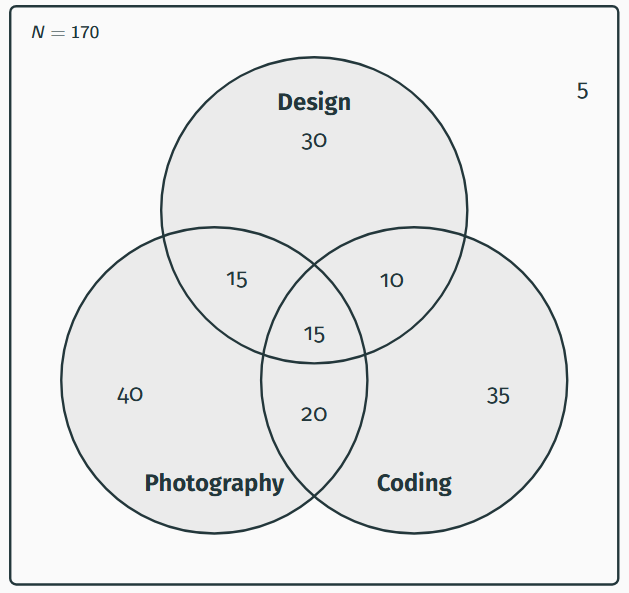
\includegraphics[width=0.9\textwidth]{img/Venn3.png}
% \end{minipage}

% % \begin{tikzpicture}[scale=1.0,baseline=(current bounding box.center)]
% %   \def\r{1.8}   % circle radius (cm)
% %   \def\dx{2.35} % horizontal distance between A and B (cm)
% %   \def\dy{2.00} % vertical offset for top circle C (cm)
% %   \def\pad{0.60} % padding between circles and rectangle (cm)

% %   % Centers of the three sets
% %   \coordinate (A) at (0,0);           % Photography
% %   \coordinate (B) at (\dx,0);         % Coding
% %   \coordinate (C) at (.5*\dx,\dy);    % Design (top)

% %   % Universe rectangle (outline only)
% %   \draw[line width=.8pt, rounded corners=2pt]
% %     (-\r-\pad,-\r-\pad) rectangle (\dx+\r+\pad,\dy+\r+\pad);

% %   % Set fills + outlines (light gray fill like your 2-set style)
% %   \fill[black!8] (A) circle (\r);
% %   \fill[black!8] (B) circle (\r);
% %   \fill[black!8] (C) circle (\r);
% %   \draw[line width=.8pt] (A) circle (\r);
% %   \draw[line width=.8pt] (B) circle (\r);
% %   \draw[line width=.8pt] (C) circle (\r);

% %   % Universe label (top-left inside the box)
% %   \node[font=\scriptsize,anchor=north west]
% %     at (-\r-\pad+0.12,\dy+\r+\pad-0.12) {$N=170$};

% %   % Set labels
% %   \node[font=\small\bfseries] at ($(A)+(0,-0.68*\r)$) {Photography};
% %   \node[font=\small\bfseries] at ($(B)+(0,-0.68*\r)$) {Coding};
% %   \node[font=\small\bfseries] at ($(C)+(0,0.7*\r)$) {Design};

% %   % ----- Region counts -----
% %   % Only Photography
% %   \node[font=\small] at ($(A)+(-0.55*\r,-0.10*\r)$) {40};
% %   % Only Coding
% %   \node[font=\small] at ($(B)+(0.55*\r,-0.10*\r)$) {35};
% %   % Only Design
% %   \node[font=\small] at ($(C)+(0,0.45*\r)$) {30};

% %   % Two-way only regions (subtracting the triple)
% %   % P ∩ C only
% %   \node[font=\small] at ($.5*(A)+.5*(B) + (0,-0.22*\r)$) {20};
% %   % P ∩ D only
% %   \node[font=\small] at ($.5*(A)+.5*(C) + (-0.18*\r,0.10*\r)$) {15};
% %   % C ∩ D only
% %   \node[font=\small] at ($.5*(B)+.5*(C) + (0.18*\r,0.10*\r)$) {10};

% %   % Triple intersection
% %   \node[font=\small] at ($.5*(A)+.5*(B) + (0,0.3*\r)$) {15};

% %   % Outside (none)
% %   \node[font=\small]
% %     at (\dx+\r+0.3*\pad, \dy+0.78*\r) {5};
% % \end{tikzpicture}

% \end{frame}


% \begin{frame}{\orange{Distributive property of sets} (+ 0.2)}
    
%     % {\hspace{3.7cm}
%     Given the sets $A, B, C$, proof that 
    
%     \begin{enumerate}[leftmargin = 0.5cm, label = (alph*), rightmargin = 0.2cm]
%         \item[(a)] $A \cup (B \cap C)$ = $(A \cup B) \cap (A\cup C)$
%         \item[(b)] $A \cap (B \cup C)$ = $(A \cap B) \cup (A\cap C)$
%         \item[(c)] $(M \backslash B) \cup (M \backslash T) = M \backslash (B \cap T)$
%     \end{enumerate}

%     \textbf{Hint:} Prove that every element of the set on the left is also an element of the set on the right and viceversa
%     % }
    
% \end{frame}

% \begin{frame}{Algebraic manipulation}

%     Perform the following algebraic manipulations:
    
%     \begin{enumerate}[leftmargin = 0.5cm, label = (\alph*), rightmargin = 0.2cm]

%     \item Simplify the expression $(-(ab^3)^{-3}(a^6b^6)^2)^3$
    
%     \item If $\lrp{\frac{xy}{z}}^{-2} = 3$, what is the value of $\lrp{\frac{z}{xy}}^{6}$?

%     \item Factor the expressions $50 - x^2$ and $a^3 - 4a^2b + 4ab^2$

%     \item Simplify the expression $\frac{x}{3-x} - \frac{1-x}{x+3} - \frac{24}{x^2 - 9}$

%     \item Reduce the fraction $\frac{4a^2 - 12ab + 9b^2}{4a^2 - 9b^2}$

%     \item Solve the inequalities $|x^2 - 4| \leq 2$ and $8 - 0.2x \leq (4 - 0.1x)/0.5$
    
%     \end{enumerate}
    
% \end{frame}

% \begin{frame}{Manipulating logarithms}

    % \begin{enumerate}[leftmargin = 0.5cm, label = \arabic*., rightmargin = 0.2cm]

    % \item Show that $a^x = \exp(x\ln(a))$ ($\exp(x)$ is the same as $e^x$)
    
    % \item Show that $\ln(a^x) = x\ln(a)$

    % \item What is the smallest $n\in\N$ such that $(2/3)^n  \leq 1/30$ \\
    % Hint: take $\ln$ in both sides and use the fact that $\ln(a^x) = x\ln(a)$

    % \item Solve the equations:
    
    % \begin{enumerate}[leftmargin = 0.5cm, label = (\alph*), rightmargin = 0.2cm]
    
    %     \item $3^x 4^{x+2} = 8$

    %     \item $3\ln(x) + 2\ln(x^2) = 6$

    %     \item $\frac{x\ln(x + 3)}{x^2 + 1} = 0$

    %     \item $4^x - 4^{x-1} = 3^{x+1} - 3^x$

    % \end{enumerate}

%     \end{enumerate}
    
% \end{frame}

% \begin{frame}{Manipulating logarithms — Solution}

% \begin{enumerate}[leftmargin=0.5cm, label=\arabic*., rightmargin=0.2cm]
%   % \item $a^x=\exp(x\ln a)$:
%   %       Let $y=\exp(x\ln a)$. Then $\ln y=x\ln a=\ln(a^x)$, so $y=a^x$ since $\ln$ is injective.

%   % \item $\ln(a^x)=x\ln a$:
%   %       $\ln(a^x)=\ln(\exp(x\ln a))=x\ln a$ by (1) and $\ln\circ\exp=\mathrm{id}$.

%   \item $n\ln(\tfrac23)\le\ln(\tfrac1{30})$ and $\ln(\tfrac23)<0$, hence
%         $n\ge\frac{\ln(1/30)}{\ln(2/3)}\approx 8.39$. Minimal $n=\boxed{9}$
%         % (since $(\tfrac23)^8\approx0.039>1/30$ and $(\tfrac23)^9\approx0.026<1/30$).

%   \item Solve:
%     \begin{enumerate}[leftmargin=0.5cm, label=(\alph*), rightmargin=0.2cm]
%       \item $3^x4^{x+2}=8 \;\Rightarrow\; 12^x\cdot16=8 \Rightarrow 12^x=\tfrac12
%             \Rightarrow x=\dfrac{\ln(1/2)}{\ln 12}=-\dfrac{1}{\log_{2}12}\approx -0.279.$
%       \item $3\ln x+2\ln(x^2)=3\ln x+4\ln x=7\ln x=6 \Rightarrow \boxed{x=e^{6/7}}\ \ (x>0).$
%       \item $\dfrac{x\ln(x+3)}{x^2+1}=0 \Rightarrow x\ln(x+3)=0
%             \Rightarrow \boxed{x=0\ \text{or}\ x=-2}$ \ (domain $x>-3$).
%       \item $4^x-4^{x-1}=3^{x+1}-3^x \Rightarrow \tfrac34\,4^x=2\,3^x
%             \Rightarrow (\tfrac43)^x=\tfrac83
%             \Rightarrow \boxed{x=\dfrac{\ln(8/3)}{\ln(4/3)}\approx 3.409.}$
%     \end{enumerate}
% \end{enumerate}
% \end{frame}


\begin{frame}{Manipulating logarithm and ``$n$-Folding'' times}

    Using the fact that $\ln(a^x) = x\ln(a)$, solve the following problems.
    
    \begin{enumerate}[leftmargin = 0.5cm, label = \arabic*., rightmargin = 0.2cm]

    \item What is the smallest $m\in\N$ such that $(2/3)^m  \leq 1/30$ \\
    
    \item The population of Zimbabwe increases $3.5\%$ every year, how much time it will take for the population to double its size?
    
    \item On average, the S\&P 500 stock market index yields $p\%$ of annual returns. If you invest in the S\&P 500, and assuming constant annual compounding with reinvestment, how long would you have to wait until your money is tripled?

    \end{enumerate}
    
\end{frame}

\begin{frame}{Manipulating logarithms and ``$n$-folding'' times — Solution}

\begin{enumerate}[leftmargin=0.5cm, label=\arabic*., rightmargin=0.2cm]
  
  \item $m\ln(\tfrac23)\le\ln(\tfrac1{30})$ and $\ln(\tfrac23)<0$, hence
        $m\ge\frac{\ln(1/30)}{\ln(2/3)}\approx 8.39$. Minimal $m=\boxed{9}$
  
  \item   
  Let $P_0$ be the initial population. After $m$ years, $P_m = P_0(1+0.035)^m$. \\
  We want to solve the equation $P_m=2P_0$:
  \[
    P_m=2P_0 \;\Longrightarrow\; 2=(1.035)^m \;\Longrightarrow\; m=\frac{\ln 2}{\ln(1.035)}\approx \boxed{20.15\text{ years}}
  \]
  % (about \(\,20\) years and \(2\) months).  

  \item 
  Wealth after $m$ years: \(W_m=W_0(1+\tfrac{p}{100})^m\).
  We need to solve \(W_m=3W_0\):
  \[
    W_m=3W_0 
    \;\Longrightarrow\;
    3=\bigl(1+\tfrac{p}{100}\bigr)^m
    \;\Longrightarrow\;
    \boxed{\,m=\dfrac{\ln 3}{\ln\!\bigl(1+\tfrac{p}{100}\bigr)}\,}
  \]
\end{enumerate}

\medskip
\centering
\textbf{General $n$-folding time at percentage $p$ per year:}\;
\(\displaystyle m=\frac{\ln n}{\ln(1+p/100)}\).
\end{frame}


% \begin{frame}{\red{Geometry, Trigonometry, and Pi:\\ the most simple relation of the most simple shape}}
    
%     Let $P_n(x)$ be the perimeter of the regular polygon of $n$ sides with side length $x$

%     \begin{enumerate}[leftmargin = 0.5cm, label = (\alph*), rightmargin = 0.2cm]

%         \item Write down the explicit dependency on $x$ of the function $P_n$
        
%         \item Proof heuristically that the sequence $P_n(2\sin((180/n)^\circ))$ converges to the perimeter of a circle with unit radius (assume that you don't know the formula of the circle's perimeter)

%         \textbf{Hint:} Inscribe regular polygons inside the circle

%         \item Define 
%         $$
%         \pi = \frac{\text{Perimeter of the circle}}{\text{Diameter of the cricle}}
%         $$
%         Find a sequence that converges to $\pi$ using the previous results
%     \end{enumerate}
    
    
% \end{frame}

% \begin{frame}{Solution}

%     \begin{enumerate}[leftmargin = 0.5cm, label = (\alph*), rightmargin = 0.2cm]

%         \item $P_n(x) = nx$
        
%         \item Using Pitagora's theorem and the fact that the sine of an angle is the ratio of the opposite and adjacent sides of an rectangle triangle, we can prove that the length of the cord of a circle with unit radius and angle...  $P_n(2r \sin((180/n)^\circ)) =  2n\sin((180/n)^\circ)$

%         \textbf{Hint:} Inscribe regular polygons inside the circle

%         \item Define 
%         $$
%         \pi = \frac{\text{Diameter of the cricle}}{\text{Perimeter of the circle}}
%         $$
%         Find a sequence that converges to $\pi$ using the previous results
%     \end{enumerate}
    
    
% \end{frame}

% \begin{frame}{\orange{Wrapping the earth}}

%     If a rope could be wrapped around the Earth’s surface at the equator, it would be approximately circular and about $40$ million meters long. Suppose we wanted to extend the rope to make it $1$ meter above the equator at every point. How many more meters of rope would be needed?
%     (Recall that the circumference of a circle with radius $r$ is $2\pi r$.)
    
% \end{frame}

\begin{frame}{\orange{Mathematical induction} (+ 0.2)}

    {\hspace{0.2cm}
    \begin{minipage}{0.6\textwidth}
    Proof that the following inequality holds for every $x \geq -1$ and every $n \in \N$:
    $$
    (1 + x)^n \geq 1 + nx
    $$
    \textbf{Hint:} approach the problem as follows:
    \begin{enumerate}[leftmargin = 0.5cm, label = \arabic*., rightmargin = 0.2cm]
        \item prove it for $n = 1$
        \item prove that if it holds for $n$ arbitrarily chosen, then does it for $n+1$
        \item conclude that the inequality holds true
    \end{enumerate}
    This approach is known as \textbf{mathematical induction} and is a handy method for proving that a statement is true for all natural numbers or any numerable set
    \end{minipage}
    \begin{minipage}{0.35\textwidth}
    
        {\hspace{0.3cm} 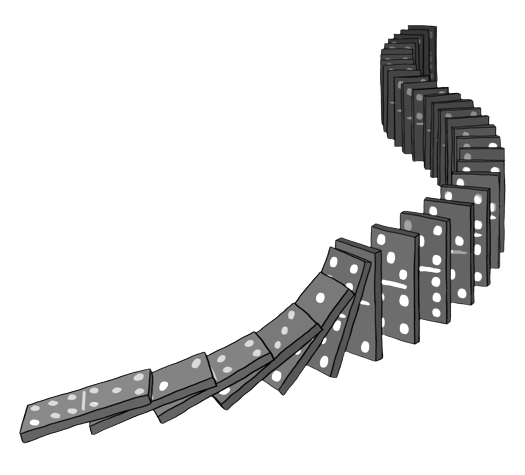
\includegraphics[width = 0.95\textwidth, height = 5.5cm]{img/induction.png}}
    \end{minipage}
    }
    
\end{frame}

\begin{frame}{Interpretation, reasoning, and modeling}

    \begin{enumerate}[leftmargin = 0.5cm, label = \arabic*., rightmargin = 0.2cm]

        \item An item initially costs a dollar and then its price is increased by $p\%$. Afterward, the (new) price is lowered by $p\%$. What is the final price of the item?
        
        \item A person buys $x_1$ , $x_2$ , and $x_3$ units of three goods whose prices per unit are respectively $p_1$ , $p_2$ , and $p_3$ . What is the total expenditure?
        
        \item Using a mobile phone costs $\$30$ per month, and an additional $\$0.16$ per minute of use.

        \begin{enumerate}[leftmargin = 0.5cm, label = (\alph*), rightmargin = 0.2cm]
            \item What is the cost for one month if the phone is used for a total of $x$ minutes?
            \item What are the smallest and largest numbers of hours you can use the phone in a month if the monthly telephone bill is to be between $\$102$ and $\$126$?
        \end{enumerate}
        
    \end{enumerate}
    
\end{frame}

\begin{frame}{Interpretation, reasoning, and modeling — Solutions}

\begin{enumerate}[leftmargin=0.5cm, label=\arabic*., rightmargin=0.2cm]

  \item \textbf{Up $p\%$, then down $p\%$.}
  \[
  1 \xrightarrow{\,+p\%\,} 1\!\left(1+\frac{p}{100}\right)
    \xrightarrow{\,-p\%\,} \left(1+\frac{p}{100}\right)\!\left(1-\frac{p}{100}\right)
    = 1-\left(\frac{p}{100}\right)^2.
  \]
  Final price: \(\boxed{1-\bigl(\tfrac{p}{100}\bigr)^2}\) dollars (a net decrease of \( \tfrac{p^2}{10{,}000}\) dollars).

  \item \textbf{Total expenditure.}
  \[
    \boxed{\,\text{Expenditure}=x_1p_1+x_2p_2+x_3p_3\,}.
  \]

  \item \textbf{Mobile plan: \$30/month + \$0.16 per minute.}
  \begin{enumerate}[leftmargin=0.5cm, label=(\alph*), rightmargin=0.2cm]
    \item For \(x\) minutes in a month:
      \[
        \boxed{\,C(x)=30+0.16\,x\quad (\text{dollars})\,}.
      \]
    \item Bill between \$102 and \$126:
      \[
        102 \le 30+0.16x \le 126
        \;\Longrightarrow\;
        72 \le 0.16x \le 96
        \;\Longrightarrow\;
        450 \le x \le 600\ \text{min}.
      \]
      In hours: \(\boxed{7.5 \le \text{hours} \le 10}\), i.e.\ smallest \(7\text{h }30\text{m}\), largest \(10\text{h }0\text{m}\).
  \end{enumerate}

\end{enumerate}
\end{frame}


\begin{frame}{Solving equations}

    1. Solve the following equations:
    
    \begin{enumerate}[leftmargin = 0.8cm, label = (\alph*), rightmargin = 0.2cm]

    \item $\frac{2x}{3} = \frac{2x - 3}{3} + \frac{5}{x}$
    
    \item $\lrp{(1-\lambda)a^{-\rho} + \lambda b^{-\rho}}^{-1/\rho} = c$, for $b$

    \item $x^2 + 2x - 35 = 0$

    \item $(x^4 + 1)(4 + x) = 0$

    \item $-x^2 + 10x = 25$
    
    \end{enumerate}

    2. For which values of $\alpha$ has the equation $x^2 + \alpha x + 1 = 0$ no solutions, exactly one solution, or two solutions? Determine the solutions in the second and third cases
    
\end{frame}

\begin{frame}{Solving equations — Solution}
\footnotesize
\begin{enumerate}[leftmargin=0.5cm, label=\arabic*., rightmargin=0.2cm]

\item Solve:
\begin{enumerate}[leftmargin=0.5cm, label=(\alph*), rightmargin=0.2cm]

  \item 
  \[
  \dfrac{2x}{3}=\dfrac{2x-3}{3}+\dfrac{5}{x} 
  \;\Leftrightarrow\; 
  2x^2=(2x-3)x+15 
  \;\Leftrightarrow\; 
  0=-3x+15 
  \;\Leftrightarrow\; 
  \boxed{x=5}.
  \]

  \item 
  \[
  \bigl((1-\lambda)a^{-\rho}+\lambda b^{-\rho}\bigr)^{-1/\rho}=c
  \;\Leftrightarrow\; 
  (1-\lambda)a^{-\rho}+\lambda b^{-\rho}=c^{-\rho}
  \;\Leftrightarrow\; 
  b^{-\rho}=\frac{c^{-\rho}-(1-\lambda)a^{-\rho}}{\lambda}.
  \]
  For $\lambda\neq0$,
  \[
  \boxed{\,b=\left(\frac{\lambda}{\,c^{-\rho}-(1-\lambda)a^{-\rho}\,}\right)^{\!1/\rho}}
  \]
  
  \item $x^2+2x-35=0 \;\Rightarrow\; (x+7)(x-5)=0 \;\Rightarrow\; \boxed{x=-7,\,5}$.

  \item $(x^4+1)(x+4)=0 \;\Rightarrow\; \boxed{x=-4}$ is the only real solution.

  \item $-x^2+10x=25 \;\Rightarrow\; x^2-10x+25=0 \;\Rightarrow\; (x-5)^2=0 \;\Rightarrow\; \boxed{x=5}$.
\end{enumerate}

\item Parameter $\alpha$ in $x^2+\alpha x+1=0$ (real solutions):
\[
\Delta=\alpha^2-4.
\]
\begin{itemize}[leftmargin=0.6cm]
  \item No real solution if $\boxed{|\alpha|<2}$.
  \item Exactly one real solution if $\boxed{|\alpha|=2}$:
        \; $\alpha=2\Rightarrow x=-1$; \; $\alpha=-2\Rightarrow x=1$.
  \item Two distinct real solutions if $\boxed{|\alpha|>2}$:
        \[
        \boxed{\,x=\dfrac{-\alpha\pm\sqrt{\alpha^2-4}}{2}\,}.
        \]
\end{itemize}

\end{enumerate}
\end{frame}


\begin{frame}{Functions}
    
    \begin{enumerate}[leftmargin = 0.5cm, label = (\alph*), rightmargin = 0.2cm]

    \item Recall that: (i) the relationship between the Celsius (C) and Fahrenheit (F) temperature scales is linear; (ii) water freezes at $0^\circ$C and $32^\circ$F; and (iii) water boils at $100^\circ$C and $212^\circ$F.

    \begin{enumerate}[leftmargin = 0.5cm, label = (\alph*), rightmargin = 0.2cm]
        \item Determine the equation that converts C to F \\
        \item Which temperature is represented by the same number in both scales?
    \end{enumerate}
    
    \item Find the equation of the parabola that passes through $(1, -3)$, $(0, -6)$, and $(3, 15)$

    \item The functions $f$, $g$, $h$ are given by $f(x) = x^2 + 1$, $g(x) = 1/x^2$, $h(x) = \sqrt{x}$. Find formulae for the compositions $f\circ g$, $g\circ f$, $h\circ f$, $f\circ h$, $h\circ f\circ g$
    
    \end{enumerate}
    
\end{frame}

\begin{frame}{Functions — Solution}
\footnotesize
\begin{enumerate}[leftmargin=0.5cm, label=(\alph*), rightmargin=0.2cm]

  \item \textbf{Celsius–Fahrenheit.}
  \begin{enumerate}[leftmargin=0.5cm, label=(\roman*), rightmargin=0.2cm]
    \item Line through \((0,32)\) and \((100,212)\).
          Slope \(m=\frac{212-32}{100-0}=\frac{180}{100}=\tfrac{9}{5}\).
          Hence \(\boxed{F=\tfrac{9}{5}C+32}\).
    \item Same number on both scales: solve \(C=F\).
          $$
          C=\tfrac{9}{5}C+32 \Rightarrow -\tfrac{4}{5}C=32 \Rightarrow \boxed{C=F=-40}.
          $$
  \end{enumerate}

  \item \textbf{Parabola through \((1,-3),(0,-6),(3,15)\).} \\
        Let \(y=ax^2+bx+c\). \\
        From \((0,-6)\): \(c=-6\). \\
        From \((1,-3)\): \(a+b-6=-3\Rightarrow a+b=3\).\\
        From \((3,15)\): \(9a+3b-6=15\Rightarrow 3a+b=7\).\\
        Solve the system for $a$ and $b$: $a=2$ and \(b=1\).
        \[
          \boxed{y=2x^2+x-6}.
        \]

  \item \textbf{Compositions of } \(f(x)=x^2+1,\ g(x)=\tfrac{1}{x^2},\ h(x)=\sqrt{x}\).
        \[
        \begin{aligned}
          (f\circ g)(x) &= f\!\left(\tfrac{1}{x^2}\right)=\tfrac{1}{x^4}+1, \quad &x\neq0.\\
          (g\circ f)(x) &= g(x^2+1)=\tfrac{1}{(x^2+1)^2}, \quad &\text{all }x.\\
          (h\circ f)(x) &= h(x^2+1)=\sqrt{x^2+1}, \quad &\text{all }x.\\
          (f\circ h)(x) &= f(\sqrt{x})=(\sqrt{x})^2+1=x+1, \quad &x\ge 0.\\
          (h\circ f\circ g)(x) &= h\!\bigl(f(g(x))\bigr)=\sqrt{\tfrac{1}{x^4}+1}, \quad &x\neq0.
        \end{aligned}
        \]
\end{enumerate}
\end{frame}



\begin{frame}{Supply-demand equilibrium}
    
    Suppose that the supply and demand sets for a particular market are 
    $$
    S = \{(q, p)\ |\ 3p - q = 5\},\quad D = \{(q, p)\ |\ 3p + q^2 + 2q = 9\}
    $$
    Sketch $S$ and $D$ and determine the equilibrium set $E = S \cap D$. Comment briefly on the interpretation of the results

\end{frame}

\begin{frame}{Supply–demand equilibrium — Solution}

\footnotesize

\begin{enumerate}[leftmargin = 0.5cm, label = $\bullet$, rightmargin = 0.2cm]
\item Write both sets as price–quantity relations (price $p$ as a function of quantity $q$):
\begin{align*}
    S:&\ 3p-q=5 \ \Longrightarrow\ p_S(q)=\frac{q+5}{3}\quad\text{(upward line)},\\    
    D:&\ 3p+q^2+2q=9 \ \Longrightarrow\ p_D(q)=\frac{9-q^2-2q}{3}=\frac{10-(q+1)^2}{3}\ \text{(downward parabola)}.
\end{align*}
\item Equilibrium points solve $p_S(q)=p_D(q)$:
\[
\frac{q+5}{3}=\frac{9-q^2-2q}{3}\;\Longrightarrow\; q^2+3q-4=0\;\Longrightarrow\; q=\boxed{1}\ \text{or}\ q=\boxed{-4}.
\]
Prices: $p=\frac{q+5}{3}$ gives $(q,p)=(1,2)$ and $(-4,\tfrac13)$. Hence
\[
\boxed{E=S\cap D=\{(1,2),\,(-4,\tfrac13)\}}.
\]
\item Interpretation: in the economically feasible quadrant $q\ge0,\ p\ge0$, the market equilibrium is unique at $\boxed{(q^*,p^*)=(1,2)}$ (quantity $1$, price $2$). The second intersection has negative quantity and is not economically meaningful.
\end{enumerate}

\end{frame}

\begin{frame}{Supply–demand equilibrium — Visualization}

\medskip
\begin{center}
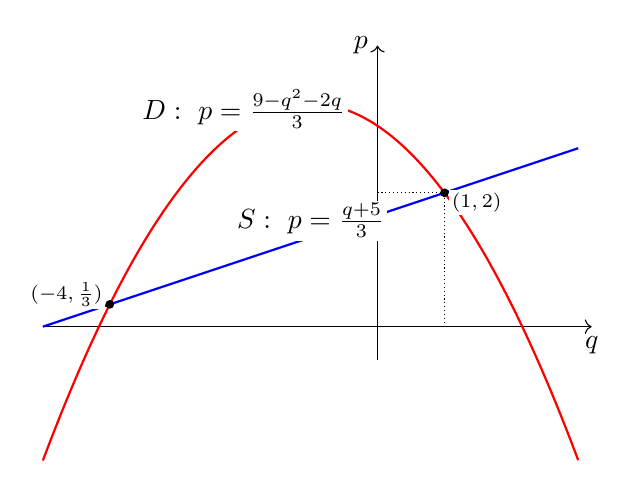
\begin{tikzpicture}[scale=0.85, baseline=(current bounding box.center)]
  % Axes window
  \def\xmin{-5}\def\xmax{3}
  \def\ymin{-0.5}\def\ymax{4}
  % Axes
  \draw[->] (\xmin,0) -- (\xmax+0.2,0) node[below] {$q$};
  \draw[->] (0,\ymin) -- (0,\ymax+0.2) node[left] {$p$};

  % Supply: p = (q+5)/3
  \draw[thick, blue] plot[domain=\xmin:\xmax, samples=200]
    (\x, {(\x+5)/3});

  % Demand: p = (9 - q^2 - 2q)/3
  \draw[thick, red] plot[domain=\xmin:\xmax, samples=200]
    (\x, {(9 - \x*\x - 2*\x)/3});

  % Labels with white chips
  \node[fill=white, inner sep=1pt] at (-1, {(-1+5)/3 + 0.25}) {$S:\ p=\frac{q+5}{3}$};
  \node[fill=white, inner sep=1pt] at (-2, {3.0 + 0.25}) {$D:\ p=\frac{9 - q^2 - 2q}{3}$};

  % Intersections
  \filldraw[black] (1,2) circle (1.6pt);
  \node[anchor=west, font=\scriptsize, fill=white, inner sep=1pt] at (1.06,1.85) {$(1,2)$};

  \filldraw[black] (-4, {1/3}) circle (1.6pt);
  \node[anchor=east, font=\scriptsize, fill=white, inner sep=1pt] at (-4.06, {0.48}) {$(-4,\tfrac{1}{3})$};

  % Dotted guides for the positive-quadrant equilibrium
  \draw[densely dotted] (1,0) -- (1,2);
  \draw[densely dotted] (0,2) -- (1,2);
\end{tikzpicture}
\vspace{0.5cm}

\href{https://www.desmos.com/calculator/t3ixeobjc2}{Visualize your own problems!}
\end{center}
\end{frame}

\begin{frame}{Sequences and limits}

    \begin{enumerate}[leftmargin = 0.5cm, label = \arabic*., rightmargin = 0.2cm]
        
        \item In $1964$ a five-year plan was introduced in Tanzania. One objective was to double the real income per capita over the next $15$ years. What is the annual rate of growth of real income per capita required to achieve this objective? Assume constant annual rate of growth.

        \item Determine the $n^{\text{th}}$ term and the limit (if it exists) of the sequence

        \begin{enumerate}[leftmargin = 0.5cm, label = (\alph*), rightmargin = 0.2cm]
            \item $-1, 3, -5, 7, -9, \dots$
            \item $1, 3, 5, 9, 17, 31, \dots$
            \item $1, 1/3, 1/9, 1/27, \dots$
            \item $0, 1/3, 0, 1/3, 0, 1/3, \dots$
        \end{enumerate}

    \end{enumerate}
    
\end{frame}

\begin{frame}{Sequences and limits — Solution}
\footnotesize
\begin{enumerate}[leftmargin=0.5cm, label=\arabic*., rightmargin=0.2cm]

  \item \textbf{Doubling in 15 years (constant annual growth).}
  \[
    (1+r)^{15}=2 \;\Longrightarrow\; r=\;2^{1/15}-1\;\approx\;\boxed{4.729\%\text{ per year}}.
  \]

  \item \textbf{$n$th term and limit.}
  \begin{enumerate}[leftmargin=0.5cm, label=(\alph*), rightmargin=0.2cm]
    \item $-1,3,-5,7,-9,\dots$ \\
          \(\displaystyle a_n=(-1)^n(2n-1)\) for $n\geq 1$. \\ 
          No limit, odd terms go to $-\infty$ and even terms go to $\infty$.

    \item $1,3,5,9,17,31,\dots$ \\
          \(\displaystyle a_n=2^{\,n-1}+1\) for \(n\ge1\); \\
          No finite limit, $a_n \rightarrow \infty$.

    \item $1,\tfrac13,\tfrac19,\tfrac1{27},\dots$ \\
          \(\displaystyle a_n=\bigl(\tfrac13\bigr)^{n-1}\). \\
          $a_n \rightarrow 0$.

    % \item $6,12,20,30,42,\dots$ \\
    %       consecutive–product pattern:
    %       \(\displaystyle a_n=a_{n-1} + 6(n-1), \, a_1 = 6\). \\
    %       No finite limit, $a_n \rightarrow \infty$.

    \item $0,\tfrac13,0,\tfrac13,0,\tfrac13,\dots$ \\
          $a_n = 0$ for $n$ odd and $a_n = 1/3$ for even $n$\, (equivalently, \(\displaystyle a_n=\frac{1+(-1)^n}{6}\)) \\
          No limit \(0\) odd terms equal $0$ and even terms equal $1/3$.

    % \item $0.9,1.1,0.99,1.01,0.999,1.001,\dots$ \\
    %     $a_{n}=1-10^{-(n+1)/2}$ for odd $n$, and $a_{n}=1+10^{-n/2}$ for even $n$. \\
    %       \(a_n \rightarrow 1\).
  \end{enumerate}

\end{enumerate}
\end{frame}


\begin{frame}{Limits}

    Find the following limits

    \begin{enumerate}[leftmargin = 0.5cm, label = (\alph*), rightmargin = 0.2cm]

        \item $\lim_{n\rightarrow\infty} \frac{n^2 + 100}{n^3 + 5}$

        \item $\lim_{n\rightarrow\infty} a^n$, for the cases $a \in (-1, 1)$, $a\leq -1$, and $a > 1$, and $a = 1$

    \end{enumerate}
    
\end{frame}

\begin{frame}{Limits — Solutions}
\begin{enumerate}[leftmargin=0.5cm, label=(\alph*), rightmargin=0.2cm]

  \item $\displaystyle \lim_{n\to\infty}\frac{n^2+100}{n^3+5}
        =\lim_{n\to\infty}\frac{\tfrac{1}{n}+ \tfrac{100}{n^2}}{1+\tfrac{5}{n^3}}
        =0$.

  \item 
  \[
  \;
  \lim_{n\to\infty} a^n 
  =
  \begin{cases}
    0, & |a|<1,\\[2pt]
    1, & a=1,\\[2pt]
    \text{diverges to }+\infty, & a>1,\\[2pt]
    \text{does not converge (oscillates),} & a=-1,\\[2pt]
    \text{no limit; }|a|^n\to\infty\text{ and signs alternate}, & a<-1.
  \end{cases}
  \]

\end{enumerate}
\end{frame}


\begin{frame}{The number $e$: compound interest}

    Write down the sequence $x_n$ in terms of $n$, where $x_n$ is the final amount of money after a year with a compound interest of $\frac{100}{n}\%$ per $\frac{1}{n}$ years and an initial investment of $\$1$ (e.g., for $n = 1$, your money is doubled after a year, for $n = 2$, you get half of your investment after six months and then half of the new compounded quantity after the other six months, and so on...)
    \vspace{0.3cm}
    
    % Which is more profitable, a $1/n$ yearly return scheme or a $1/(n+1)$ one?
    % \vspace{0.3cm}
    
    Compute the terms relative to yearly returns ($n = 1$), monthly returns ($n = 12$), weekly returns ($n = 52$) and daily returns ($n = 360$). Comment on the results
    
\end{frame}

\begin{frame}{The number $e$: compound interest — Solution}
\footnotesize
Initial investment \$1. Each period is $1/n$ years with interest rate $(100/n)\%$ per period, i.e.\ rate $r=\tfrac{1}{n}$.

\medskip
\textbf{Sequence.} After $n$ periods in one year,
\[
\boxed{\,x_n=\bigl(1+\tfrac{1}{n}\bigr)^{n}\,}.
\]

% \textbf{Which scheme is more profitable? $1/n$ or $1/(n{+}1)$?}
% \[
% \frac{x_{n+1}}{x_n}
% =\frac{(1+\frac{1}{n+1})^{n+1}}{(1+\frac{1}{n})^{n}}
% =\Bigl(1-\frac{1}{(n+1)^2}\Bigr)^{\!n}\cdot\Bigl(1+\frac{1}{n+1}\Bigr).
% \]
% Using Bernoulli’s inequality $(1-x)^n\ge 1-nx$ for $x\in[0,1]$,
% \[
% \frac{x_{n+1}}{x_n}\ \ge\ \Bigl(1-\frac{n}{(n+1)^2}\Bigr)\Bigl(1+\frac{1}{n+1}\Bigr)
% =\frac{(n^2+n+1)(n+2)}{(n+1)^3}
% =\frac{n^3+3n^2+3n+2}{(n+1)^3}\;>\;1.
% \]
% Hence $\boxed{x_{n+1}>x_n}$, so the $\tfrac{1}{n+1}$-yearly scheme yields \emph{more} than the $\tfrac{1}{n}$ one.

\medskip
\textbf{Numerics (one year, \$1 initial):}
\[
\begin{array}{lcl}
\text{Yearly }(n=1): & x_1=(1+1)^1 = \boxed{2.000000} \\
\text{Monthly }(n=12): & x_{12}=(1+\tfrac{1}{12})^{12} \approx \boxed{2.613035} \\
\text{Weekly }(n=52): & x_{52}=(1+\tfrac{1}{52})^{52} \approx \boxed{2.692597} \\
\text{Daily }(n=360): & x_{360}=(1+\tfrac{1}{360})^{360} \approx \boxed{2.714516}
\end{array}
\]

\medskip
\textbf{Comment.} Returns rise with more the more-frequent-less-gains compounding scheme. The limit is
\[
\lim_{n\to\infty}\bigl(1+\tfrac{1}{n}\bigr)^n = \boxed{e \approx 2.7182818}.
\]
\end{frame}


% \begin{frame}{\red{Formal definition of real numbers}}

%     A real number can be expressed as $a.a_1a_2a_3\dots$, with $a\in \Z$ and $a_n\in\{0, 1, 2, \dots 9\}$. Based on this representation:
%     \vspace{0.3cm}
        
%     \begin{enumerate}[leftmargin = 0.5cm, label = (\alph*), rightmargin = 0.2cm]
        
%         \item Conclude that real numbers can be expressed as the limit of rational numbers
    
%         \item Use the concept of limit to propose a formal definition for the set of real numbers $\R$
%     \end{enumerate}
    
% \end{frame}

\begin{frame}{Income, consumption, and investment}

    A closed economy produces an income $Y_n$ in year $n$ of which a part $C_n$ is consumed and the remainder $I_n$ is invested; thus 
    $$
    Y_n = C_n + I_n
    $$
    It is believed that consumption $C_n$ in year $n$ is one-half of the current year's income. %; that is, $C_n = Y_n/2$ . 
    It is also believed that next year's income is proportional to the current investment. %; that is, Y t+l = kIt, where k is a constant.
    
    Show that investment $I_n$ satisfies a first-order recurrence equation, and find the condition for the investment (and income) to rise from year to year.
    
\end{frame}

\begin{frame}{Income, consumption, and investment — Solution}

Given
\[
Y_n=C_n+I_n,\qquad C_n=\tfrac12 Y_n,\qquad Y_{n+1}=k\,I_n\quad (k>0).
\]

\textbf{Recurrence.} From $C_n=\tfrac12 Y_n$,
\[
I_n=Y_n-C_n=\tfrac12 Y_n.
\]
Using now that $Y_{n}=k\,I_{n-1}$ we get
\[
I_n=\frac{k}{2}I_{n-1}.
% Y_{n+1}=k\,I_n=k\cdot\tfrac12 Y_n=\tfrac{k}{2}\,Y_n
% \quad\Longrightarrow\quad
% \boxed{\,I_{n+1}=\tfrac{k}{2}\,I_n\,}\quad
% \text{(since }I_{n+1}=\tfrac12 Y_{n+1}\text{)}.
\]

\textbf{Solution for the $n$th term in terms of $I_0$.}
\[
I_n=\Big(\tfrac{k}{2}\Big)^n I_0\,.
\]

\textbf{Growth condition.} Year-to-year increase iff
\[
\frac{I_{n+1}}{I_n}=\tfrac{k}{2} \;>\;1
\;\Longleftrightarrow\;
\boxed{\,k>2\,}.
\]
If $k=2$: income is constant; if $0<k<2$: it declines to $0$.
\end{frame}

\begin{frame}{Linear cobweb model} 

    Suppose that the supply and demand sets for a certain good are
    $$
    S = \{(q, p)\ |\ q = 4p - 6\}, \quad D = \{(q, p)\ |\ q = 10 - 5p\}.
    $$
    
    Assuming that the suppliers operate according to the cobweb model, that is, if $p_t$ and $q_t$ are (respectively) the price and quantity in year $t$, then $p_t = p_D(q_t)$ and $q_t = q_S(p_{t-1})$. 

    \begin{enumerate}[leftmargin = 0.5cm, label = (\alph*), rightmargin = 0.2cm]
    
        \item Find the equilibrium set $E = S \cap D$. Is it economically feasible?

        \item Write down the first-order recurrence equations for $p_t$ and $q_t$

        \item Express $p_t$ and $q_t$ in terms of $t$
    
        \item How does $p_t$ and $q_t$ behave as $t$ tends to infinity?
    
    \end{enumerate}
    
\end{frame}

\begin{frame}{Linear cobweb model — Solution}
\footnotesize
Supply: $q_S(p)=4p-6$. \; Demand (inverse): from $q=10-5p$ we get $p_D(q)=2-\tfrac{q}{5}$.

\begin{enumerate}[leftmargin=0.5cm, label=(\alph*), rightmargin=0.2cm]
  \item \textbf{Equilibrium $E=S\cap D$.}
  \[
    4p-6=10-5p \;\Rightarrow\; 9p=16 \Rightarrow p^*=\tfrac{16}{9},\qquad
    q^*=4p^*-6=\tfrac{10}{9}.
  \]
  Hence $\boxed{E=\{(\tfrac{10}{9},\,\tfrac{16}{9})\}}$, economically feasible since $q^*,p^*>0$.

  \item \textbf{Cobweb recurrences.}
  \[
    \boxed{\,q_t=4p_{t-1}-6,\qquad p_t=2-\tfrac{1}{5}q_t\,}.
  \]
  Eliminating $q_t$ (price-only):
  \[
    \boxed{\,p_t=\tfrac{16}{5}-\tfrac{4}{5}\,p_{t-1}\,}.
  \]
  Eliminating $p_t$ (quantity-only):
  \[
    \boxed{\,q_{t+1}=2-\tfrac{4}{5}\,q_t\,}.
  \]

  \item \textbf{Solution.}
  \[
    p_t-p^*=(-\tfrac45)^t\,(p_0-p^*),\qquad
    q_t-q^*=(-\tfrac45)^t\,(q_0-q^*).
  \]
  % In terms of $p_0$ only (for $n\ge1$): \quad
  % $q_n=q^*+4(-\tfrac45)^{n-1}(p_0-p^*)$. \\
  % In terms of $q_0$ only: \quad
  % $p_n=p^*-\tfrac{1}{5}(-\tfrac45)^{n}(q_0-q^*)$.

  \item \textbf{Long-run behavior.}
  The multiplier is $-\dfrac{4}{5}$ with magnitude $<1$, so $p_n\to p^*$ and $q_n\to q^*$.
\end{enumerate}
\end{frame}

\begin{frame}{Linear cobweb model - Visualization}

\centering
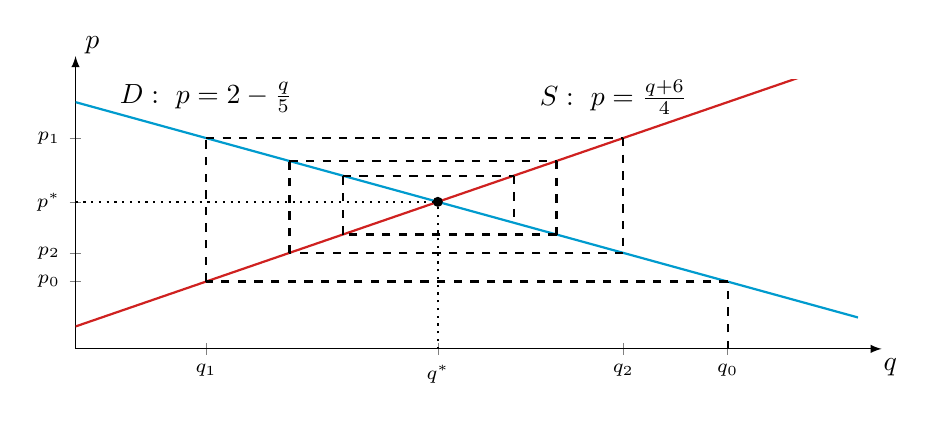
\begin{tikzpicture}
\begin{axis}[
    width=0.95\textwidth,
    height=5.0cm,
    axis lines=middle,
    xmin=0, xmax=2.4,
    ymin=1.45, ymax=2.05,
    xtick={0.4,1.111111,1.68,2.0},
    xticklabels={$q_1$,$q^*$,$q_2$,$q_0$},
    ytick={1.6,1.664,1.777778,1.92},
    yticklabels={$p_0$,$p_2$,$p^*$,$p_1$},
    ticklabel style={font=\scriptsize},
    xlabel={$q$},
    ylabel={$p$},
    axis line style={-latex,shorten >=-0.3cm},
    xlabel style={at={(ticklabel* cs:1)}, xshift=0.2cm, anchor=north west},
    ylabel style={at={(ticklabel* cs:1)}, yshift=0.2cm, anchor=south west},
]

  % Supply and demand (in p(q) form)
  \addplot[thick, firebrick3, samples=200, domain=0:2.4] {0.25*x + 1.5};
  \addplot[thick, deepskyblue3, samples=200, domain=0:2.4] {2 - 0.2*x};

  % Labels for curves
  \node[inner sep=1pt] at (axis cs:1.65,2.01) {$S:\ p=\frac{q+6}{4}$};
  \node[inner sep=1pt] at (axis cs:0.4,2.01) {$D:\ p=2-\frac{q}{5}$};

  % Equilibrium point (q*, p*)
  \addplot[only marks, mark=*, mark size=1.6pt] coordinates {(1.111111,1.777778)};

  % Cobweb (start at q0=2 -> p0=1.6)
  \draw[dashed, thick] (axis cs:2.0,1.45) -- (axis cs:2.0,1.6);     % up to p0 on D
  \draw[dashed, thick] (axis cs:2.0,1.6)  -- (axis cs:0.4,1.6);     % across to S -> q1
  \draw[dashed, thick] (axis cs:0.4,1.6)  -- (axis cs:0.4,1.92);    % to p1 on D
  \draw[dashed, thick] (axis cs:0.4,1.92) -- (axis cs:1.68,1.92);   % to S -> q2
  \draw[dashed, thick] (axis cs:1.68,1.92)-- (axis cs:1.68,1.664);  % to p2 on D

  % ---- extra iterations (q3,p3) ... (q6,p6) ----
  \draw[dashed, thick] (axis cs:1.68,1.664)      -- (axis cs:0.656,1.664);       % q3
  \draw[dashed, thick] (axis cs:0.656,1.664)     -- (axis cs:0.656,1.8688);      % p3
  \draw[dashed, thick] (axis cs:0.656,1.8688)    -- (axis cs:1.4752,1.8688);     % q4
  \draw[dashed, thick] (axis cs:1.4752,1.8688)   -- (axis cs:1.4752,1.70496);    % p4
  \draw[dashed, thick] (axis cs:1.4752,1.70496)  -- (axis cs:0.81984,1.70496);   % q5
  \draw[dashed, thick] (axis cs:0.81984,1.70496) -- (axis cs:0.81984,1.836032);  % p5
  \draw[dashed, thick] (axis cs:0.81984,1.836032)-- (axis cs:1.344128,1.836032); % q6
  \draw[dashed, thick] (axis cs:1.344128,1.836032)--(axis cs:1.344128,1.7311744);% p6

  % Guides to equilibrium
  \draw[dotted, thick] (axis cs:1.111111,1.45) -- (axis cs:1.111111,1.777778);
  \draw[dotted, thick] (axis cs:0,1.777778)    -- (axis cs:1.111111,1.777778);

\end{axis}
\end{tikzpicture}

    
\end{frame}


\begin{frame}{\orange{The general linear case of the cobweb model} (+0.2)} 

    Suppose that the supply and demand sets for a certain good are
    $$
    S = \{(q, p)\ |\ q = bp - a\}, \quad D = \{(q, p)\ |\ q = c - dp\},
    $$
    with $b, d \in \R_+$, and $a, c \in \R$
    
    Assuming that the suppliers operate according to the cobweb model, that is, if $p_t$ and $q_t$ are (respectively) the price and quantity in year $t$, then $p_t = p_D(q_t)$ and $q_t = q_S(p_{t-1})$. 

    \begin{enumerate}[leftmargin = 0.5cm, label = (\alph*), rightmargin = 0.2cm]
    
        \item Find the equilibrium set $E = S \cap D$. Is it economically feasible?

        \item Write down the first-order recurrence equations for $p_t$ and $q_t$

        \item Express $p_t$ and $q_t$ in terms of $t$
    
        \item How does $p_t$ and $q_t$ behave as $t$ tends to infinity?
    
    \end{enumerate}
    
\end{frame}

% \begin{frame}{\orange{The general linear cobweb — Solution}}
% \tiny
% Supply: $q=bp-a$; Demand: $q=c-dp$ with $b,d>0$. Inverse demand $p_D(q)=\dfrac{c-q}{d}$ and supply rule $q_S(p)=bp-a$.
% \medskip

% \begin{enumerate}[leftmargin=0.5cm, label=(\alph*), rightmargin=0.2cm]
% \item \textbf{Equilibrium $E=S\cap D$.}  Solve $bp-a=c-dp$:
% \[
% p^*=\frac{a+c}{b+d},\qquad q^*=bp^*-a=\frac{bc-ad}{\,b+d\,}.
% \]
% So $\boxed{E=\{(q^*,p^*)\}}$ (a single point).

% \item \textbf{Recurrences.} Cobweb timing: $q_t=q_S(p_{t-1})$, $p_t=p_D(q_t)$:
% \[
% \boxed{\,q_t=bp_{t-1}-a,\qquad p_t=\frac{c-q_t}{d}
%       =\frac{a+c}{d}-\frac{b}{d}\,p_{t-1}\,}.
% \]
% Equivalently, a $q$-only recursion: $\displaystyle \boxed{\,q_t=\frac{bc-ad}{d}-\frac{b}{d}\,q_{t-1}\,}$.

% \item \textbf{Closed forms (deviations from equilibrium).}
% Let $\beta=\dfrac{b}{d}>0$. Then
% \[
% p_t-p^*=-(\beta)\,(p_{t-1}-p^*) \;\Rightarrow\; 
% \boxed{\,p_t=p^*+(-\beta)^t\,(p_0-p^*)\,}.
% \]
% Similarly
% \[
% q_t-q^*=-(\beta)\,(q_{t-1}-q^*) \;\Rightarrow\;
% \boxed{\,q_t=q^*+(-\beta)^t\,(q_0-q^*)\,}.
% \]
% (Also $q_t=q^*+b\,(-\beta)^{t-1}(p_0-p^*)$ for $t\ge1$.)

% \item \textbf{Asymptotics.} Since the multiplier is $-\beta=-\dfrac{b}{d}$:
% \[
% \begin{cases}
% \boxed{b<d}: & |-\beta|<1 \Rightarrow (p_t,q_t)\to(p^*,q^*) \text{ with alternating oscillations;}\\
% \boxed{b=d}: & |-\beta|=1 \Rightarrow \text{perpetual 2-cycle about }(p^*,q^*);\\
% \boxed{b>d}: & |-\beta|>1 \Rightarrow \text{divergent oscillations (instability).}
% \end{cases}
% \]
% \emph{Interpretation:} Convergence requires the supply slope to be smaller than the (absolute) demand slope.
% \end{enumerate}
% \end{frame}


\end{document}
